\documentclass[a4paper, DIV20, 12pt, headsepline, parskip, flushleft]{scrartcl}
\usepackage[utf8]{inputenc}
\usepackage[onehalfspacing]{setspace}
\usepackage{enumerate}
\usepackage{amsmath}
\usepackage{amssymb}
\usepackage{mathtools}
\usepackage{fancyhdr}
%\usepackage{natbib}
\usepackage{graphicx}
\usepackage{listings} 
\usepackage{tikz}
\usepackage{pdfpages}
\usepackage{listings}
\usepackage{xstring}
\usepackage{etoolbox}
\usepackage[ngerman]{babel}
\usepackage{wrapfig}
\usepackage{float}
\usepackage{url}

%%% Bib %%%
\usepackage[backend=bibtex]{biblatex}
\usepackage[babel,german=quotes]{csquotes}
\usepackage{xpatch}
\bibliography{quellen}
%%% /Bib %%%
\usetikzlibrary{arrows,automata,positioning,calc}
\pagestyle{fancy}
\begin{document}
\author{Lukas Glitt}
\title{Festplatten}
\date{\today}
\maketitle
\thispagestyle{empty}
\setcounter{page}{1}
\begin{abstract}
Es wird die historische, sowie technische Entwicklung der Festplatte erläutert. Im weiteren werden Technik und Funktion moderner Festplatten beschrieben. Im Zusammenhang werden die wichtigsten Hersteller, sowie gängige Anschlusstechnologien erläutert. 
\end{abstract}
\newpage
\tableofcontents
\thispagestyle{empty}
\setcounter{page}{1}
\newpage
\section{Einführung}
Die folgende Ausarbeitung beschäftigt sich mit der Technik von Speichersystemen, auf Basis von magnetischen Speichermedien, in Form von Festplatten. Hierbei wird kurz auf die historische Entwicklung der Festplatte eingegangen. Der Schwerpunkt liegt darauf folgend auf der Technik und den Aufbau von Festplatten. Im nachfolgenden wird auf die Anschlusstechnologien und Protokolle, sowie auf die wesentlichen Hersteller eingegangen. Hierbei wird auch ein Ausblick auf die SSD als aufkommender Konkurrent zur klassischen Festplatte gegeben. Im Fazit wird ein Ausblick auf die Zukunftsfähigkeit und weiteren technischen Möglichkeiten der Festplatte gegeben. 

\subsection{Definition}
"` Eine Festplatte (auch HDD) ist ein Laufwerk, das Daten magnetisch auf mehreren, im Gehäuse untergebrachten, Scheiben speichert und auf diese wahlfreien (=beliebigen) Zugriff bietet."' \textsuperscript{ \cite{clk}}
\section{Geschichte}
\subsection{Die Vorläufer der Festplatte}
In der Datenverarbeitung werden lange Zeit vor der ersten Festplatte Lochkarten und Bandlaufwerke als Speichermedien eingesetzt. 
Diese haben den entscheidenden Nachteil, dass diese sehr hohe Zugriffszeiten aufweisen und zeitgleich nur eine sehr geringe Speicherdichte bieten können.
Dieses Problem führen bei der US-Airforce dazu nach einer Alternative zu suchen und so wird die Firma IBM mit der Suche nach einer Lösung beauftragt. \textsuperscript{\cite{ccm}}
\subsection{Die erste Festplatte und ihre anfängliche Entwicklung}
\begin{wrapfigure}{r}{0.4\textwidth}
	\vspace{-50pt}
	\begin{center}
    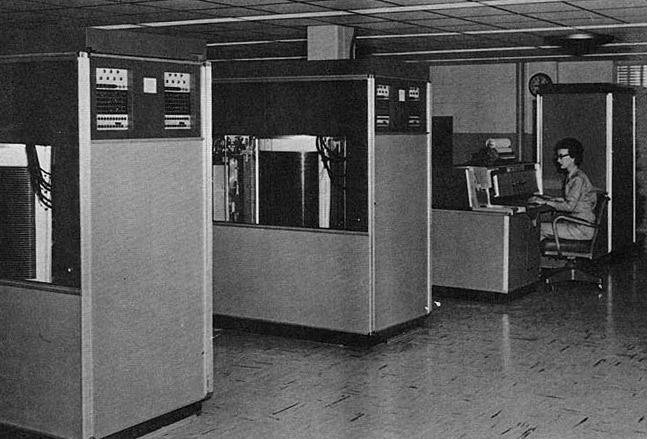
\includegraphics[width=0.35\textwidth]{RAMAC.jpeg}
    \end{center}
    \vspace{-20pt}
	\caption{IBM 305 RAMAC \textsuperscript{\cite{img:ramac}}}
     \vspace{-70pt}
\end{wrapfigure} 
Die erste Festplatte wurde 1956 von der Firma IBM unter dem Namen Ramac 305 auf den freien Markt gebracht. Ramac steht hier als Abkürzung für "Radmon Access Method of Acounting and Control". Diese bietet mit 50 Scheiben à 61 cm Durchmesser eine nie zuvor gesehene Datendichte und Zugriffsgeschwindigkeit. Auf dem Datenträger können bis zu 5MB bei einer Übertragungsrate von 8,8 KB/s gespeichert werden.
Der für damalige Verhältnisse nahezu mit 600ms in Echtzeit stattfindende Zugriff auf die Daten sorgt für eine hohe Akzeptanz der Festplatte als Datenspeicher.
Es werden über 1000 Stück des Ramac 305 hergestellt und zu damals 3200 Dollar angeboten. Dies entspricht an der heutigen Kaufkraft gemessen um die 27.000 Dollar monatlich.\textsuperscript{ \cite{ccm} \cite{epv} \cite{hhdd}}\newline
Mit dem IBM 3111 drive wird 1962 die erste Festplatte auf dem Markt eingeführt, welche wechselbare Speicherplatten bietet und somit einen gewissen Rahmen an Mobilität der Daten ermöglicht.
1973 wird ebenfalls von IBM das Winchester Projekt gestartet. Das Ergebnis dessen ist mit dem IBM 3340 ein Speicher, in welchem die rotierenden Scheiben fest montiert sind und eine Speicherkapazität von 30 MB geboten wird.\textsuperscript{\cite{hdd}}\newline
1979 wird die 8 Zoll Winchester auf den Markt gebracht. Diese bekommt 1980 massive Konkurrenz, durch die ST506 von Seagate, welche mit ihren verhältnismäßig kompakten 5,15 Zoll einen jahrelang gültigen Industriestandard schafft. Der PC von IBM und der erste Apple Computer lassen die Nachfrage nach Festplatten in haushaltsgebräuchlichen Größen drastisch anwachsen.
Mit SCSI wird 1986 ein erstes standardisiertes Protokoll zur Ansteuerung von Festplatten definiert. Bis zu diesem Zeitpunkt müssen Festplatten mittels prioritärer Anschlüsse der Hersteller und Host Controller Karten angesprochen werden. \textsuperscript{\cite{hdd}}\newline
Mit ATA 1989 und später SATA als zwei weiteren Standards wird die Grundlage einer zukunftsfähigen Anschlussmöglichkeit für Festplatten in den folgenden Jahren geschaffen. Gerade SATA ist hier als serielles Protokoll bedeutend, da dieses die Arbeit mit vielen Festplatten ermöglicht und auch die immer größer werdenden Datenmengen bewältigen kann. Im Jahr 2004 kommt die erste Festplatte mit SATA Interface auf den Markt und das 1997 eingeführte Nutzung GMR bei Lese-/Schreibköpfen wird im laufe der Zeit der allgemeine Standard. Mittlerweile entwickelt sich mit der 2,5 Zoll Festplatte ein weiterer Standard, welcher überwiegend für die Verwendung in mobilen Geräten, wie Laptops konzipiert ist. \newline
In den folgenden Jahren setzt sich das Wachstum bei den maximal möglichen Speichermengen pro Festplatte rasant fort und 2007 wird die magische Grenze von einem Terabyte seitens Hitachi geknackt. 2009 sind die ersten 2 Terabyte Festplatten verfügbar und ein Jahr darauf schon 3 TB.\newline
Ab 2015 gelangt man zu dem Schluss, dass Luft einen zu hohen Widerstand im Inneren der Festplatte darstellt und es wird Helium in Festplatten verwendet, welches noch einmal eine Erhöhung der Speichermenge auf heute über 10TB pro Festplatte ermöglichte.\textsuperscript{\cite{hgsthel}}

\section{Aufbau und Funktion}

\subsection{Formfaktoren}
Festplatten sind in verschiedenen Formfaktoren anzutreffen. Heute haben sich dabei zwei Formfaktoren primär durchgesetzt. Die 2.5"' und 3.5"' Festplatte. Die 3.5 Zoll Festplatten werden überwiegend in Desktopcomputern und Servern eingesetzt. Die 2.5 Zoll Modelle werden in der Regel in Laptops eingebaut, aber erfreuen sich aber auf Grund ihrer geringen Größe und mittlerweile beachtlichen Speichergrößen  einer immer weiter wachsenden Beliebtheit im Serversegment. Als letzte heute noch verwendeten Formfaktor gilt es die 1.8"' Festplatten zu nennen. Diese werden überwiegend in Notebooks, Netbooks und noch kleineren Geräten eingesetzt, welche keinen Flashspeicher verwenden.
3.5"' Festplatten können mittlerweile bis zu 10TB Daten fassen. Bei 2.5"' liegt dieser Wert momentan bei 5TB. 
1.8"' Festplatten kommen hier auf maximal 250GB Speicher.
\textsuperscript{\cite{gza}\cite{gzb}\cite{gzc}}

Ergänzend zu diesen drei Formfaktoren waren früher noch 5.25"', 1"' und 0.85"' Festplatten in Verwendung. Diese setzen sich aber nicht auf dem Markt durch und sind heute nicht mehr verfügbar.

\subsection{Die Komponenten}
Eine Festplatte besteht neben dem Gehäuse aus diversen Komponenten. Die wichtigsten dabei sind die magnetischen Scheiben, der Motor, die Lese- und Schreibköpfe, sowie der Controller. Die folgende Grafik gibt einen Überblick über die wichtigsten Bauteile einer Festplatte.
\begin{figure}[H]
\begin{center}
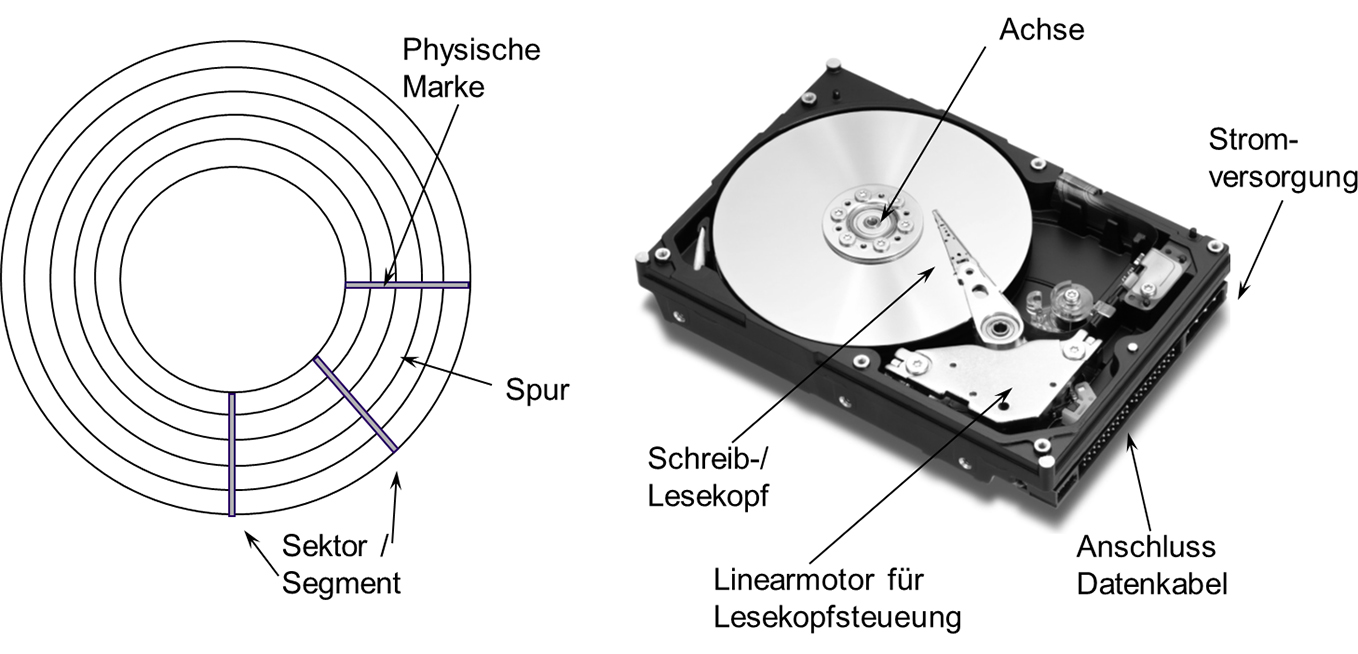
\includegraphics[scale=1.1]{hddoverview.jpg}
\end{center}
\caption{Die einzelnen Bauteile der Festplatte und Bereiche der Scheiben im Überblick\textsuperscript{\cite{img:hdd}}}
\end{figure} 
\subsubsection{magnetischen Scheiben}
Die magnetischen Scheiben, im engl. auch Platters genannt, speichern die eigentlichen Daten.
Sie rotieren innerhalb des Festplattengehäuses um ihre eigene Achse.
Von ihnen sind in einer Festplatte zwischen 3 bis 12 Scheiben verbaut. 
Diese bestehen aus einem nicht magnetischen Grundmaterial. Bei diesen ist es wichtig, dass diese sich nicht bei thermischer Energie, also Hitzeeinwirkung oder bei mechanischer Einwirkung verformen. Dafür wird gerne auf Glas oder Magnesium als Material zurückgegriffen, da diese nicht Anfällig für Verformungen sind und gleichzeitig eine geringe elektrische Leitfähigkeit aufweisen.
Eisenoxid oder Kobalt werden auf die Platten als Deckschicht aufgetragen. Die durchschnittliche Dicke beträgt dabei einen Mikrometer. Diese magnetische Schickt wird zusätzlich noch mit einer Schicht aus Carbon, also Kohlenstoff überzogen, um sie vor physischen Einwirkungen zu schützen.
In der Regel werden Ober- und Unterseite der Scheibe zum Speichern von Daten genutzt.
Es gibt zwei primär eingesetzte Techniken zur Datenspeicherung. Beide werden in den folgenden Abschnitten behandelt. Die eine ist, das seit 1970 verwendete Longitudinal Recording.
Seit 2010 wird aber, das seit 2000 immer weiter entwickelte Perpendicula Recording primär bei Festplatten eingesetzt. 
\paragraph{Longitudinal Recording}
Das Longitudinal Recording stammt aus den 60er und 70er Jahren des letzten Jahrhunderts. Diese Technik findet auch Einsatz beim Aufzeichnen von Ton auf einem Tonband. Hierbei richtet der Schreibkopf die Magnetpartikel horizontal zueinander aus. 
Dieses Verfahren erreichte bereits früh seine maximale Ausreizung bei der Speicherdichte. Dies begründet sich daraus, dass einzelne Datenbits ihre Ausrichtung auf Grund des supermagnetischen Effekts verlieren, wenn die einzelnen Datenbits zu nah beieinander liegen. 
\begin{figure}[H]
\begin{center}
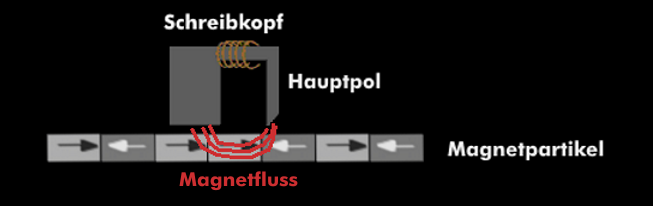
\includegraphics[scale=0.5]{prinzip-des-longitudinal-recording-lmr.png}
\end{center}
\caption{Longitudinal recoding \textsuperscript{\cite{img:lmr}}}
\end{figure}

\paragraph{Perpendicular Recording}
Das perpendicular Recording ist der direkte Nachfolger des Longitudinal Recording. Hier werden entgegen zum vorherigen Prinzip, die magnetischen Speicherbereiche vertikal angeordnet. Dies erlaubt eine bedeutend höhere Speicherdichte. Das Verfahren ist seit 1976 bekannt und wurde erstmal 1998 von IBM technisch umgesetzt. Marktreif ist das Verfahren, aber erst seit 2005. Die vertikale Anordnung der Magnetpartikel wird durch ein tieferes Eindringen des magnetischen Flusses in das Material erreicht. Um dies sauber umzusetzen wird der Schreibkopf entsprechend angepasst. Der Hauptpol(siege Abbildung 3) wird schmaler und länger. Dafür wird der Rückpol entsprechend breiter, sodass der Magnetfluss sich dort auffächern kann und so die Datenbits nicht wieder durch diesen beeinflusst werden. Vorher waren mit Longitudinal Recording höchstens Datendichten von 15 bis 30 Gigabit pro Quadratzentimeter möglich. Mit Perpendicular Recording hingegen liegt dieser Wert bei 150 Gigabit pro Quadratzentimeter. Die erste Festplatte mit dieser Technik wurde 2005 von Toshiba für die breite Masse verfügbar gemacht.  \textsuperscript{\cite{pr}\cite{pr1}}
\begin{figure}[H]
\begin{center}
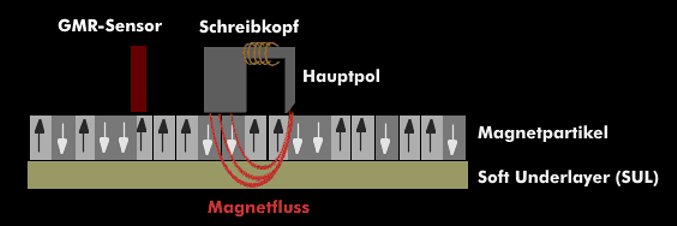
\includegraphics[scale=0.5]{prinzip-des-perpendicular-recordings.png}
\end{center}
\caption{Longitudinal recoding \textsuperscript{\cite{img:pr}}}
\end{figure}
\subsubsection{Navigation auf den Scheiben}
Um sich eindeutige Positionen auf den verschiedenen Platten zu haben gibt es ein System, dass es erlaubt an Hand der Angaben von Seiten, Zylinder, Spuren, Sektoren und Blöcken immer eine genaue Position zu bestimmen. Somit wird eine Art Koordinatensystem gebildet.
\paragraph{Seiten} beschreiben auf welcher Seite der wievielten Scheibe man sich befindet. Diese werden fortlaufend nummeriert, wobei jeweils die Ober- und Unterseite einer Scheibe mit einbezogen wird.
\paragraph{Spuren} beschreiben eine Kreisbahn mit einem festen Radius um den Mittelpunkt einer Scheibe.
\paragraph{Zylinder} bezeichnen mehrere über die Scheiben verteilt übereinander liegende Spuren.
\paragraph{Blöcke} sind die Einheiten in die eine Spur zerlegt werden kann. Jeder Block umfasst 4096 Byte.
\paragraph{Sektor} nennt man den Bereich von Blöcken, welche im gleichen Winkelbereich einer Seite liegen.

Durch diese verschiedenen Ortsangaben kann sehr genau bestimmt werden, wann von wo gelesen werden muss und macht nochmal den Unterschied zu einem linearen Speichermedium klar. Dort kann nur der komplette Inhalt nacheinander eingelesen werden, bis man zum gewünschten Punkt gelangt. Eine Festplatte hingegen ist in der Lage die Position direkt anzusteuern und die Daten entsprechend auszulesen. \textsuperscript{\cite{vid:hdd}}

\subsubsection{Motor und Rotationsgeschwindigkeit}
Der Motor bewegt den Schreib- und Lesekopf, sowie die Scheiben.
Die Scheiben werden vom Motor auf Geschwindigkeiten zwischen 5400 bis 10.000 Umdrehungen die Minute gebracht.
Hierbei ist es außerordentlich relevant, dass diese Geschwindigkeit exakt eingehalten wird, da sonst das Timing beim Auslesen der Datenbits durch den Schreib- und Lesekopf nicht mehr stimmt. 
Festplatten im 2.5 Zoll Format laufen in der Regel bei 5400 Umdrehungen pro Minute, sind aber auch mit 7400 RPM verfügbar. Bei 3.5 Zoll Desktop Festplatten ist mittlerweile 7400 Umdrehungen der Standard. Im Big Data und Serverbereich kommen in der Regel Karten mit 10.000 Umdrehungen pro Minute zum Einsatz, damit diese, die dort benötigten Schreib- und Leseraten liefern können. \textsuperscript{\cite{elk}}

\subsubsection{Lese-/Schreibkopf}
Der Lese- und Schreibkopf ist ein sehr feiner Elektromagnet, welcher zum Manipulieren der einzelnen Datenbits auf den magnetischen Scheiben verwendet wird. Heutzutage bewegt sich der Kopf in einem Abstand von 3nm über die Magnetscheiben. Dies wird mit Hilfe des Bodeneffekts erreicht. Die durch die Rotation in Bewegung gesetzte Luft, strömt dabei unter dem Kopf entlang und hält diesen dabei auf einem konstanten Abstand zu den Scheiben.
Ursprünglich wurde etwa bis zum Jahr 1994 die Daten mittels Induktion in der Spule des Lese- und Schreibkopfes ausgelesen. Dies ist ab einer gewissen Speicherdichte nicht mehr praktikabel und es musste zu empfindlicheren Leseköpfen gewechselt werden. Dabei wurden zwei Typen im Laufe der Zeit entwickelt. MR- und GMR-Leseköpfe.
GMR-Leseköpfe sind die Weiterentwicklung der MR Leseköpfe. Im folgenden wird der heute gängige GMR-Lesekopf erläutert.
\paragraph{GMR-Lesekopf}
Der GMR Lesekopf basiert auf dem Riesenmagnetowiderstand. Dieser wurde 1988 von Pro. Dr. Peter Grünberg vom Forschungszentrum Jülich und Prof. Dr. Albert Fert aus Paris entdeckt. Davor wurden diese beiden 2007 mit dem Nobelpreis für Physik ausgezeichnet.\textsuperscript{\cite{nbp}}
Der Riesenmagnetowiderstand(kurz GMR-Effekt) beschreibt das Verhalten von Strukturen, welche aus einigen Nanometern dünnen Schichten aus abwechselnd magnetischen und nicht magnetischen Materialien bestehen. Der elektrische Widerstand dieser Strukturen hängt von der gegenseitigen Orientierung der Magnetisierung der magnetischen Schichten ab. Sind diese entgegengesetzt zu einander magnetisiert, dann ist der elektrische Widerstand bedeutend höher. Der elektrische Widerstand dieser Schichten reagiert sehr empfindlich auf äußere Einflüsse. Dies macht diesen Effekt optimal zum Einsatz mit einem Sensor, wie in diesen Fall dem Lesekopf.
Beim Lesen wird durch GMR die Abtastung durch den Sensor bedeutend feiner. Dies geschieht durch den Spannungsabfall der im Sensor durch die sich drehende Magnetisierung in den Schichten auf der jeweiligen Scheibe. \textsuperscript{\cite{gmr} \cite{nbp}}
\subsubsection{Controller}
Festplattencontroller, auch Host-Bus-Adapter genannt sind in der Regel auf der Unterseite einer Festplatte in Form eines PCBs zu finden. Der Controllerbegirff stammt aus einer Zeit in welcher noch Controller Karten in Rechnern getrennt zur Ansteuerung der einzelnen Hardwarebestandteile verbaut wurden. Der Host-Bus-Adapter übernimmt die Kommunikation mit dem Mainboard-Bus und dem Betriebssystem. Der Controller verwaltet ebenfalls welche Daten, in welcher Reihenfolge, ausgelesen und gecached werden. Am Controller PCB liegt auch die Stromversorgung an. Die Datenanbindung erfolgt über eines der im nächsten Abschnitt erläuterten Protokolle bzw. Schnittstellen.
Man sieht gut in der nachfolgenden Grafik die verschiedenen Bestandteile des PCBs auf dem der Controllerchip liegt.
Vorne liegen zwei Anschlüsse. Der breite Anschluss ist in diesem Fall für SATA Strom. Der kurze ist für die SATA Datenverbindung. Direkt dahinter liegt der in diesem Fall schwarze Contollerchip. Dieser ist wiederum über Leiterbahnen mit dem Motor und dem Lese- und Schreibkopf verbunden.\textsuperscript{\cite{ctrl}}
\begin{figure}[H]
\begin{center}
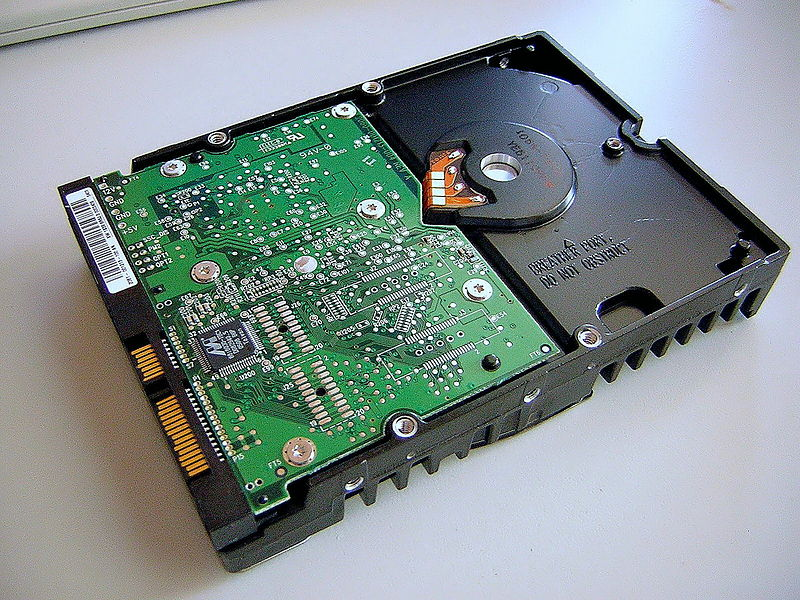
\includegraphics[scale=1]{FestplatteUnterseite.jpg}
\end{center}
\caption{Unterseite einer Festplatte \textsuperscript{\cite{img:hdddown}}}
\end{figure}
\subsection{Ablauf eines Schreib- und Lesevorgangs}
Bei Schreib- und Lesevorgängen auf Festplatten werden nicht mehr direkt die Bytes auf der Platte angesteuert, sondern immer die jeweiligen Sektoren in denen diese Bytes liegen. Somit werden z.B. immer Sektoren von 4096 Byte eingelesen. Dies sorgt aber auch dafür, dass immer nur komplette Blöcke geschrieben und gelesen werden können.
\subsubsection{Schreibvorgang}
Beim Schreibvorgang sind verschiedene relevante Schritte zu durchlaufen, bis das eigentliche Schreiben durchgeführt werden kann. Im ersten Schritt werden die erhaltenden Daten mit Fehlerkorrekturinformationen ergänzt. Dies erlaubt die Wiederherstellung des Blocks, sollte es im Betrieb zu Schäden an den Blöcken kommen.
Hierbei kommen Verfahren aus der Vorwärtsfehlerkorrektur zum Einsatz, welche darauf basieren, dass ein Teil der Daten redundant mit übergeben wird und somit eine Rekonstruktion der restlichen Daten möglich ist. \newline
Nachdem den Blöcken Fehlerkorrekturinformationen hinzugefügt worden, wird im nächsten Schritt eine Modulation des Ganzen durchgeführt, um ein für den Schreibkopf nutzbares analoges Signal zur Verfügung zu haben.
Jetzt ist der Punkt erreicht, an dem der Schreibkopf in die nähe der jeweiligen Spur gebracht wird. Hier werden Positionsmarkierungen auf den Scheiben ausgelesen und eine Feinpositionierung vorgenommen, um mittig auf der Spur anzulegen und ein Beschädigen der Nachbarspuren zu vermeiden. Ist diese Position erreicht wird der Block auf die ihm zugewiesenen Position auf der Spur geschrieben. Anschließend fährt de Kopf zur nächsten Position weiter, um die nächste Operation zu beginnen oder begibt sich in eine Warteposition.\textsuperscript{\cite{lpbus} \cite{hdd}}
\subsubsection{Lesevorgang}
Der Lesevorgang läuft im groben umgekehrt zum Schreibvorgang ab.
Hierbei wird dann eine Datei von Betriebssystem beim Controller angefordert. Daraufhin fährt der Lesekopf an die entsprechende Postion und wartet darauf bis der gewünschte Block den Kopf in seiner Rotation passiert und liest diesen aus. Nach dem Auslesen wird mittels der beigefügten Fehlerkorrekturinformationen die Daten auf Konsistenz überprüft. Da in der Regel die umgebenden Sektoren mitgelesen werden, werden diese im Cache zwischengespeichert, da die Wahrscheinlichkeit für deren nachfolgende Anforderung in der Regel sehr hoch ist.\newline
Sollte der Sektor nicht lesbar, bzw. nicht rekonstruierbar sein, wird ein CRC-Fehler zurückgemeldet. Sollten die Daten rekonstruierbar sein, aber der Sektor an sich beschädigt, werden diese an eine neue Position umgeschrieben.

\subsubsection{Festplattenscheduling}

Die Schreib- und Leseoperationen müssen organisiert und vorausgeplant werden, um zu lange Laufwege und zu hohe Reaktionszeiten zu vermeiden. Dazu kommen verschiedene Verfahren wie FCFS, SSTF, Scan oder C-Scan zum Einsatz.
Beispielhaft werden im folgenden zwei verschiedene Scheduling Ansätze kurz erläutert.\textsuperscript{\cite{lpbus}}
\paragraph{FCFS} First Come First Server arbeitet alle Anfragen in der Reihenfolge ihres Eintreffens ab. Dies sorgt für sehr viele Laufwege des Lese- und Schreibkopfes ist aber das am einfachsten umzusetzende Verfahren.
\paragraph{SSTF} Shortest Seek Time First bearbeitet die Anfragen an Hand der Lage der Sektoren zu einander. Man versucht hier immer den kürzesten Weg zwischen allen Sektoren zu finden, welche für die aktuell noch offenen Anfragen angesteuert werden müssen.

\section{Anschlusstechniken und Protokolle}
Nachdem früher die Verwendung von externen Controllerkarten zur Ansteuerung der Festplatte üblich waren, hat man diese heute in die Festplatte integriert und Anschlussmöglichkeiten an dieser selbst geschaffen, um direkt mit dem Mainboard des Computers verbunden zu werden.
Früher wurden überwiegend parallele Protokolle zur Übertragung eingesetzt. Dies stieß aber mit der Zeit an die Grenzen der Zuverlässigkeiten bei steigenden Datenraten. Daraufhin fand ein Wechsel zu seriellen Übertragungsmethoden statt. Im folgenden werden die wichtigsten Standards die heute auch immer noch zum Einsatz kommen erläutert.\textsuperscript{\cite{hdd}}
\subsection{IDE}
IDE, auch ATA genannt ist ein paralleles Übertragungsverfahren für Speichergeräte.
Bei ATA befinden sich in der Regel zwei Anschlüsse auf dem Mainboard, wobei an jeden jeweils bis zu zwei Festplatten angeschlossen werden können. Damit dies funktioniert müssen an den jeweiligen Festplatten Master/Slave Jumper gesetzt werden, damit die Geräte einwandfrei adressiert werden können. Die verschiedenen möglichen Konfigurationen für die Jumper einer ATA Festplatte werden in der nachfolgenden Grafik dargestellt.
\begin{figure}[H]
\begin{center}
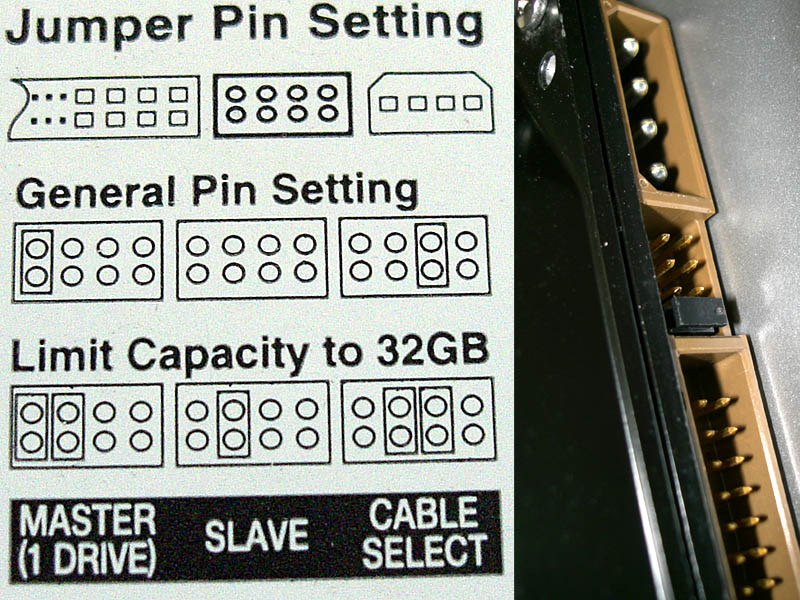
\includegraphics[scale=0.3]{IDEJumper.jpg}
\end{center}
\caption{Jumperkonfiguration an einer IDE Festplatte \textsuperscript{\cite{img:idejumper}}}
\end{figure}
Zusätzlich zu der Limitierung bei den maximal verwendbaren Festplatten kommt noch das Problem, dass die verschiedenen Geräte sich die Bandbreite an einem Kabel teilen können. Zusätzlich können auch noch CD Laufwerke mittels IDE bzw ATA angeschlossen werden, wobei aber immer zu beachten ist, dass das langsamste Gerät andere Geräte ausbremst.\newline
Ein ATA Datenkabel besteht aus einem 80 adrigen Flachbandkabel mit einem 39-Pin-Stecker.
\subsection{PSCSI}
Das Parallel Small Computer System Interface verfolgt einen ähnlichen Ansatz wie ATA. Hier sind jedoch die Vorteile, dass abhängig von den verwendeten Controllern bis zu 15 Geräte an einer parallelen Anbindung genutzt werden können. Dafür weisen ältere PSCSI Festplatten mehrere Jumperfelder auf, wo hingegen moderne PSCSI Festplatten die Adressierung automatisch übernehmen. \\
Die Möglichkeit ein einzelnes System mit bedeutend mehr Datenträgern bestücken zu können macht PSCSI vor allem für professionelle Einsatzzwecke interessant, wobei PCSCI heute genauso wie ATA größtenteils von seriellen Verfahren verdrängt wurde.
\subsection{SATA}
SATA ist der serielle nachfolger des ATA Standards und wurde 2000 von Intel entwickelt. Er bietet drei entschiedene Vorteiele gebenüber ATA. Zum einen sind bedeuten höhere Übertragungsraten möglich. Der aktuelle Standard SATA3 erreicht theoretisch bis zu 6GB/s, wobei die realistisch erreichbaren Datenraten deutlich darunter liegen. 
Im weiteren ist es möglich Geräte im laufenden Betrieb zu tauschen. Dies nennt sich HotPlug und ist im professionellen Umfeld sehr relevant, da dies ermöglicht defekte Festplatten im laufenden Betrieb zu ersetzen ohne einen Server eine Zeit lang abschalten zu müssen. 
Als letzter relevanter Vorteil ist die stark vereinfachte Kabelführung zu nennen. SATA verwendet Punkt zu Punkt Verbindungen und es ist so problemlos möglich ein einzelnes Kabel zu jedem einzelnen Datenträger führen. 
\subsection{SAS}
Serial Attached SCSI ist eine serielle Weiterentwicklung des PSCSI Standards. Hierbei werden wie bei SATA die Geräte nicht mehr über einen eigenen Bus sondern über dedizierte Ports oder Multiplier angesteuert.
SAS ist abwärtskompatibel zu SATA. Also können SATA Festplatten an jedem SAS Controller verwendet werden. Umgekehrt ist das jedoch nicht möglich. SAS Festplatten benötigen zwingend einen SAS Controller.\newline
SAS Festplatten werden fast ausschließlich im Serverbereich eingesetzt. Daher bieten diese meistens höhere Umdrehungszahlen und sind bedeutend lauter als ihre SATA Äquivalente. 
\begin{figure}[H]
\begin{center}
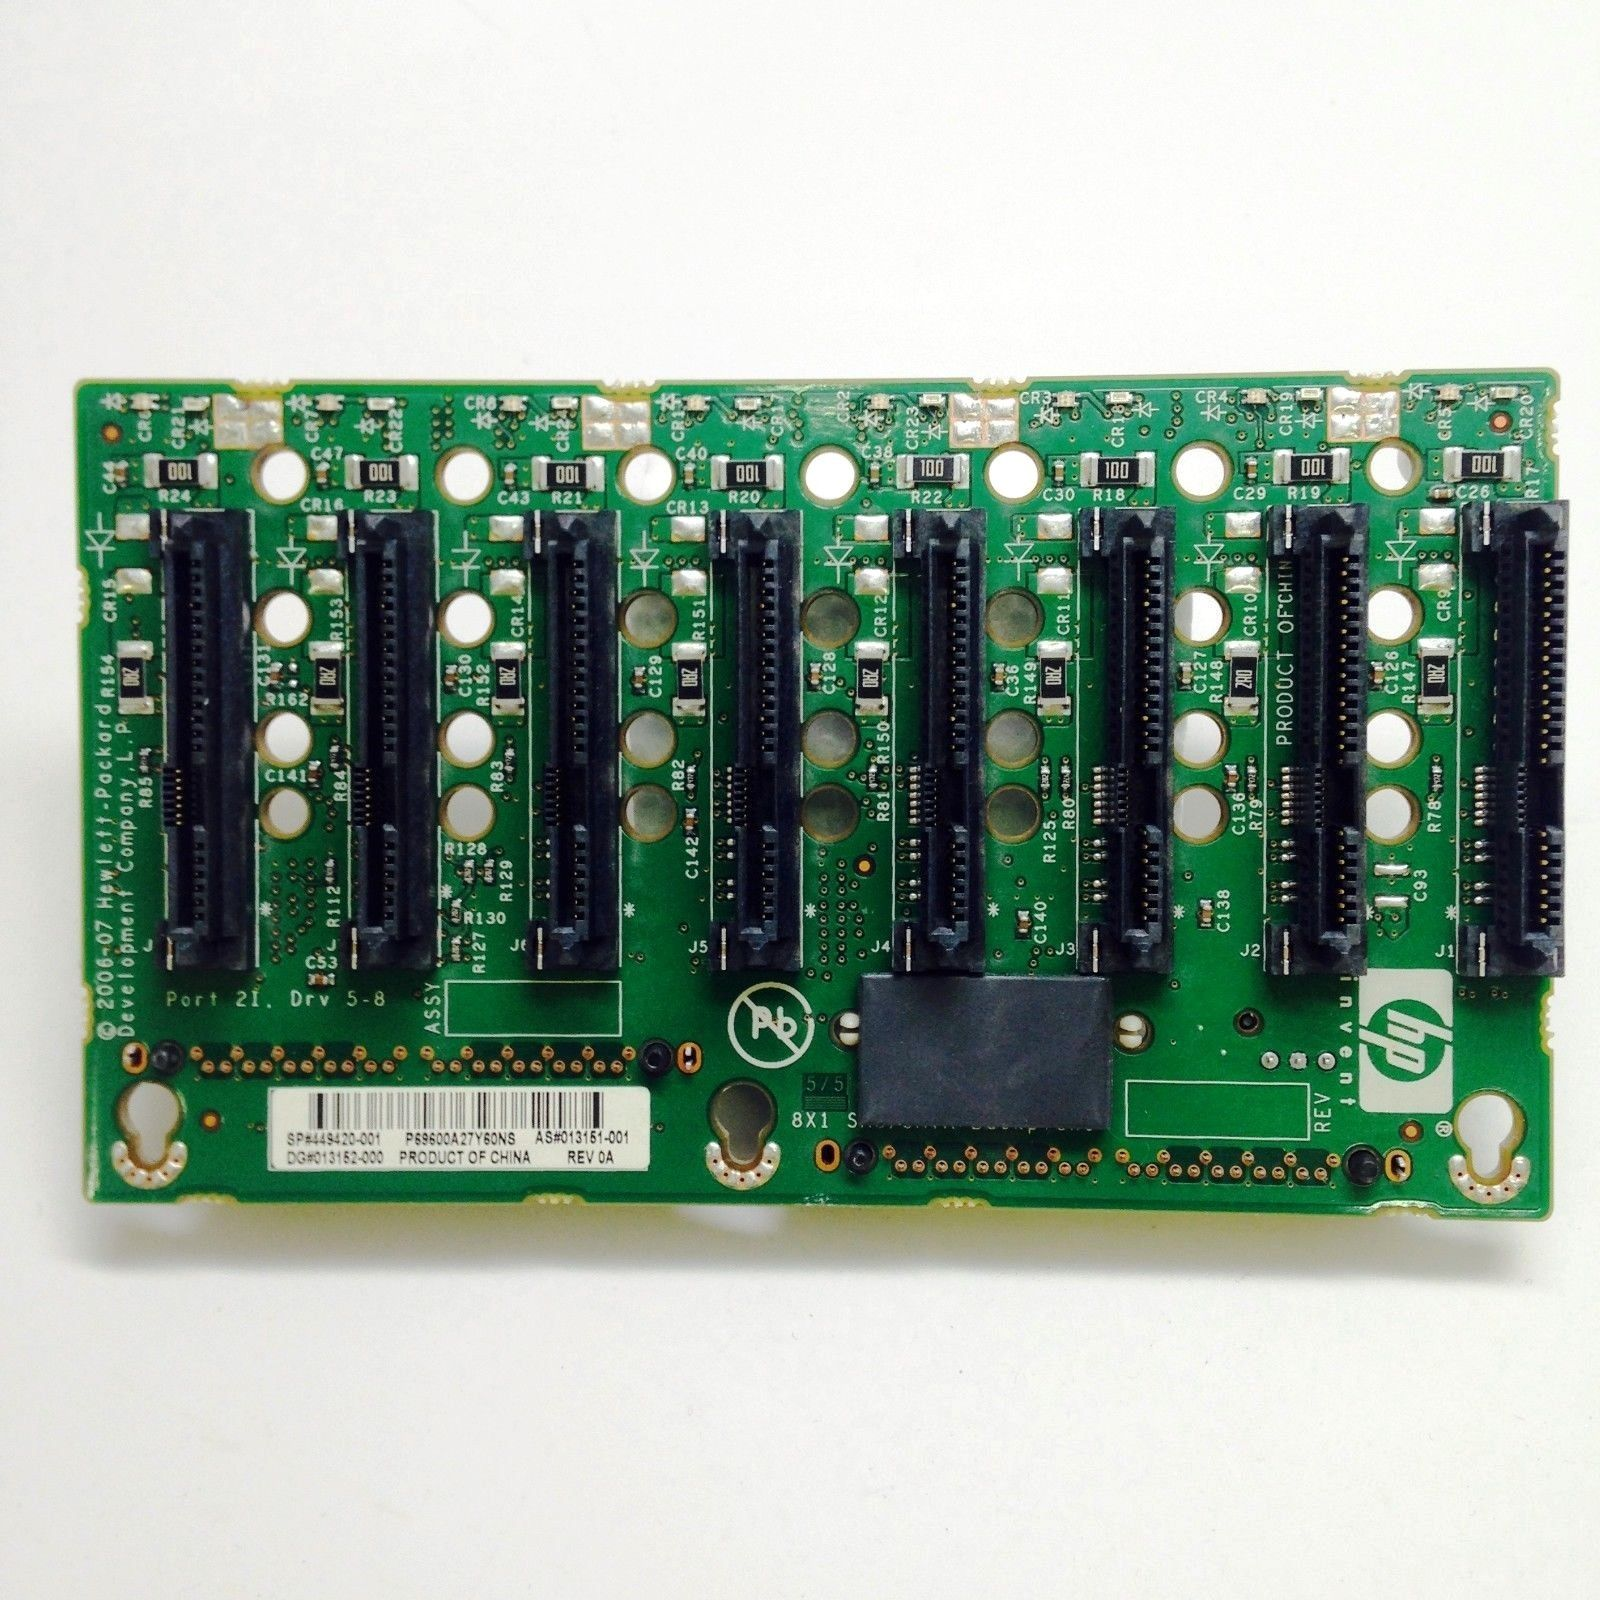
\includegraphics[scale=0.15]{sasbackplane.jpg}
\end{center}
\caption{SAS Backplane HP Server \textsuperscript{\cite{img:sas}}}
\end{figure} 
\subsection{Fibre Channel}
Festplatten mit Fibre Channel Anschluss sind für die Bewältigung großer Datenmengen Konzipiert und bieten Übertragungsraten von bis zu 16 Gbit/s. Das Protokoll zur Übertragung von Daten von und zu diesen Festplatten heißt FC-P. \newline
Sie werden häufig in SANs(Storage Area Network) verwendet. Dort sind die einzelnen Festplatten untereinander über Kupfer in einem Storagesystem angebunden und dann mittels Glasfaserverbindung mit anderen Storage Systemen verbunden. Sie stellen ihre Speicherkapazität über das Netzwerk zur Verfügung. Da diese Storage Lösungen meistens sehr viele Systeme, gerade in Kombination mit der immer weiter fortschreitenden Virtualisierung, sehr schnell mit großen Datenmengen versorgen müssen, wird hier auf Glasfasern zum maximieren der Übertragungsleistung  zurückgegriffen. 
\begin{figure}[H]
\begin{center}
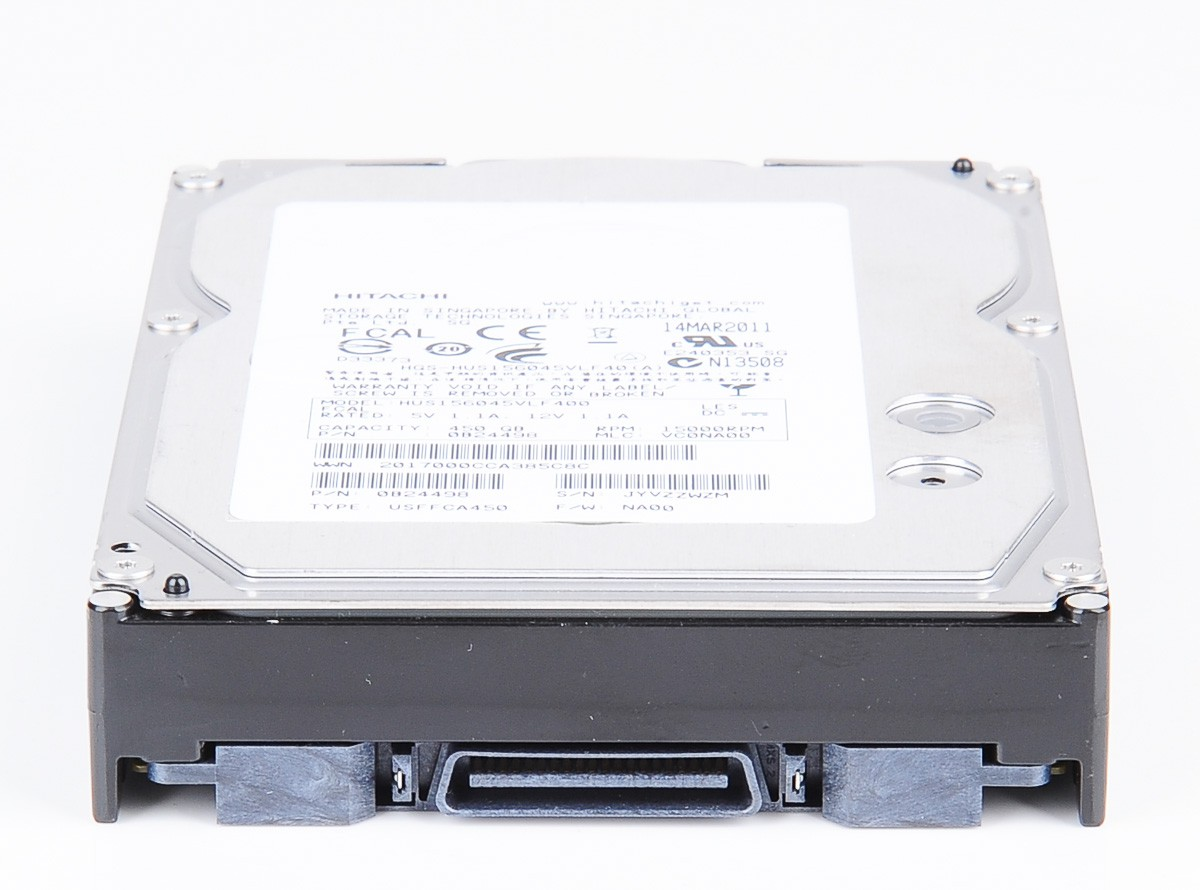
\includegraphics[scale=0.18]{fibreChannel.jpg}
\end{center}
\caption{Festplatte mit Fibre Channel Anschluss \textsuperscript{\cite{img:fibre}}}
\end{figure} 
\section{Funktionen und Einsatzgebiete}
In den vorherigen Abschnitten wurde bereits immer wieder kurz auf einzelne Einsatzgebiete von Festplatten eingegangen. Dieser Abschnitt wird nochmal die einzelnen Einsatzgebiete präzisieren und den Unterschied zu flüchtigen Speichermedien und optischen Datenträgern und Bandspeichern herausstellen. \newline


\subsection{Privatbereich}
Im privaten Umfeld werden Festplatten häufig als Speichermedien für PCs verwendet. Hierbei werden sie entweder fest im Gehäuse verbaut oder über eine externe Schnittstelle über einen Adapter wie zum Beispiel USB verbunden oder mit Hilfe eines NAS über das Netzwerk bereit gestellt.
Hierbei kommen mittlerweile fast nur noch SATA Festplatten zum Einsatz. \newline
Die klassische CD ist auf Grund Ihrer geringen Speichermenge und schlechten Performance mittlerweile fast komplett verdrängt worden. Durch die heutzutage sehr hohen Speichermengen auf Festplatten werden diese häufig als Ablageorte für große Datenmengen wie Videos, Musik oder Bilder verwendet. \newline Flashbasierte Speichermedien treten hier aber mittlerweile in eine starke Konkurrenz zu der klassischen Festplatte. Mehr dazu wird im Abschnitt 5.3 erläutert.
\subsection{Professioneller Bereich}
Im professionellem Bereich, werden Festplatten als Speichermedien für Workstations und Server genutzt.
Bei Workstations erfüllen sie dabei ähnliche Aufgaben, wie bei den Desktop PCs privater Anwender.
Im Serverbereich hingegen werden Festplatten entweder direkt in Servern als Datenspeicher verbaut oder werden anderen Servern als Speicher über das Netzwerk zur Verfügung gestellt. Beispielhaft kann man hier sehr Leistungsfähige Virtualisierungsserver nennen. Diese verfügen in der Regel über sehr große Rechenkapazitäten und sehr viel Arbeitsspeicher, aber über kaum bis gar keinen persistenten Speicher in Form von Festplatten. Dieser wird dann über das Netzwerk von Storagesystemen oder Storageservern an diese übertragen.
Es gibt mittlerweile Unternehmen, die sich darauf spezialisiert haben Festplattenspeicher über das Netzwerk anderen zur Verfügung zu stellen. Dies nennt man Storage as a Service(SaaS). 
\subsection{Die Konkurrenz durch SSDs}
SSDs sind Speichermedien auf Basis von Flashspeichern. Die Abkürzung SSD steht für Solid-State-Disk. Verschiedene Formen von SSDs existieren seid den 1970er Jahren. Die heutige Form der SSD exisitert aber erst seit 1991. Dort wurde die erste SSD für den Einsatz beim Militär und in Flugzeugen auf den Markt gebracht. Für den normalen Massenmarkt wurde SSDs ab ca 2007 verfügbar. Sie liegen preislich deutlich über dem Preis von Festplatten.  Teilweise kommt es hier bis um den Faktor 10 höhere Preise pro Gigabyte. \newline
SSDs werden in der Regel über das SATA Interface angesprochen und liegen im 2,5 Zoll Format vor. Alternativ gibt es sie auch als Steckkarten für den PCI-E oder M2 Slot. Trotz ihres höheren Preises bietet die SSD einige Vorteile gegenüber der Festplatte. Zum einen besitzt sie keinerlei mechanische Bauteile, sodass sie bedeutend unempfindlicher gegenüber äußeren Einwirkungen sind. Durch den Wegfall von beweglichen Komponenten sind die Zugriffszeiten und Übertragungsraten bedeutend höher und die Zugriffszeiten zeitgleich kleiner. Hinzu kommt, dass der Stromverbrauch durch die Abwesenheit eines Motors bedeutend kleiner ausfällt.\newline
Nachteilig gegenüber Festplatten ist die bedeutend geringere Datendichte die momentan noch auf SSDs erreicht wird. Hierbei zeichnet sich in den letzten Jahren ein rasantes Wachstum ab, sodass mittlerweile SSDs mit bis zu 4 TB auf dem Markt sind. \newline
Häufig werden SSDs mittlerweile als Hauptdatenspeicher in Workstations und Dekstop PCs, sowie Laptops eingesetzt. Dort kann das Betriebssystem von der hohen Performance der SSD profitieren und ist nicht auf sehr viel Speicher zum Unterbringen von Daten angewiesen. Häufig wird diese dann durch eine HDD ergänzt, welche als Ablageort für diverse Mediendateien und andere Daten mit großer Platzerfordernis dient.\newline
Durch die immer weiter fallenden Preise für Flash Speicher entwickelt sich die SSD zu einem ernstzunehmenden Konkurrenten zur Festplatte. \textsuperscript{\cite{ssd}}
\subsection{Vorteile und Nachteile von Festplatten}
Festplatten haben sich im Laufe vieler Jahre, in vielen Einsatzgebieten bewährt und etabliert. Dennoch haben sie einige entscheidende Nachteile, die man bei ihrem Einsatz berücksichtigen sollte.\newline
Die in Festplatten verbauten Motoren, Scheiben und Lese-/Schreibköpfe sind mechanische Bauteile. Daher unterliegen sie einem normalen Verschleiß und sind empfindlich gegenüber äußeren Einwirkungen.
Trotz verschiedener Schutzmaßnahmen im Gehäuse sind z.B. Festplatten höchst empfindlich gegen Stürzen, wenn der Schreibkopf sich nicht in der Parkposition befindet. 
Ein wichtiger Nachteil, der zu großen Problem führen kann, ist, dass Festplatten auf Grund der magnetischen Speichertechnik gegenüber magnetischen Felder anfällig sind. So kann man mit einem starken Magneten schnell aus Versehen eine Festplatte löschen.
\newline
Zu den Vorteilen von Festplatten gehören ihre hohe Datendichte und Langlebigkeit.
Sie sind sehr günstig herzustellen und häufig wieder neu beschreibbar. Grundlegend weisen Sie dazu die Eigenschaft auf nicht linear komplett eingelesen werden zu müssen, dass ihnen vor allem einen Vorteil gegenüber bandbasierten Speichern und Lochkarten verschafft.
\section{Hersteller}
Der Markt für die Herstellung von Festplatten teilt sich mittlerweile nur noch in drei große Teilnehmer auf.
Hierbei hält Western Digital mit seiner Tochter HGST zusammen den größten Anteil von 43\%. An zweiter Stelle steht Seagate als großer Hersteller mit einem Marktanteil von 41\%. Als dritten kleinen Anbieter gibt es noch Toshiba mit einem Marktanteil von 16\% im Jahre 2014. \newline
Frühere Hersteller sind fast alle in den drei heutigen Marktteilnehmern aufgegangen.
Alle drei Hersteller sind auch im Markt für SSDs aktiv. Wobei dieser Markt durch weitere Anbieter wie Samsung ergänzt wird.\newline
Im Enterprise Bereich wird überwiegend auf Festplatten von Western Digital gesetzt. Western Digital bietet verschiedene Modellreihen an, welche auf verschiedene Aufgaben spezialisiert sind. Z.B gibt es die WD Red Modelle welche besonders auf den Dauerbetrieb in NAS Systemen optimiert sind. WD Black Festplatten hingegen sind dann beispielsweise auf möglichst hohe Lese- und Schreibraten optimiert, weisen dafür aber eine etwas geringere Lebensdauer im Dauerbetrieb auf.
\textsuperscript{\cite{hdd} \cite{hddprod}}
\section{Fazit}
Die Festplatte hat eine lange Entwicklung hinter sich gebracht. Sie ist seit 1956 im Einsatz und immer noch aus der heutigen Welt nicht wegzudenken. Die Festplatte als persistentes Speichermedium für die breiten Massen hat die Digitalisierung wie sie in den letzten Jahrzehnten stattgefunden hat mit möglich gemacht. \newline
Sie erlaubt es den immer weiter wachsenden Datenmengen Herr zu werden. 
Es gibt mittlerweile flashbasierte Speichermedien welche den Festplatten in manchen Märkten Konkurrenz bereiten, aber auch dagegen behauptet sich die Festplatte als zuverlässiges und langlebiges Speichermedium. Nachteile, wie die starke Anfälligkeit gegenüber physischen externen Einflüssen wurden durch z.B. automatische Systeme zur Erkennung von Stürzen auf ein Minimum reduziert.\newline
Ich gehe davon aus, dass die Festplatte noch langfristig als wichtiger Bestandteil unserer Speicherinfrastruktur erhalten bleibt und sich neben der SSD mit Ihrem Stärken behaupten wird.
\newpage
\printbibliography[
heading=bibintoc,
title={Literatur- und Quellenverzeichnis}
]
\end{document}


